%  LaTeX support: latex@mdpi.com
%  For support, please attach all files needed for compiling as well as the log file, and specify your operating system, LaTeX version, and LaTeX editor.

%=================================================================
\documentclass[metals,article,submit,pdftex,moreauthors]{Definitions/mdpi}
% For posting an early version of this manuscript as a preprint, you may use "preprints" as the journal and change "submit" to "accept". The document class line would be, e.g., \documentclass[preprints,article,accept,moreauthors,pdftex]{mdpi}. This is especially recommended for submission to arXiv, where line numbers should be removed before posting. For preprints.org, the editorial staff will make this change immediately prior to posting.

%--------------------
% Class Options:
%--------------------
%----------
% journal
%----------
% Choose between the following MDPI journals:
% acoustics, actuators, addictions, admsci, adolescents, aerobiology, aerospace, agriculture, agriengineering, agrochemicals, agronomy, ai, air, algorithms, allergies, alloys, analytica, analytics, anatomia, animals, antibiotics, antibodies, antioxidants, applbiosci, appliedchem, appliedmath, applmech, applmicrobiol, applnano, applsci, aquacj, architecture, arm, arthropoda, arts, asc, asi, astronomy, atmosphere, atoms, audiolres, automation, axioms, bacteria, batteries, bdcc, behavsci, beverages, biochem, bioengineering, biologics, biology, biomass, biomechanics, biomed, biomedicines, biomedinformatics, biomimetics, biomolecules, biophysica, biosensors, biotech, birds, bloods, blsf, brainsci, breath, buildings, businesses, cancers, carbon, cardiogenetics, catalysts, cells, ceramics, challenges, chemengineering, chemistry, chemosensors, chemproc, children, chips, cimb, civileng, cleantechnol, climate, clinpract, clockssleep, cmd, coasts, coatings, colloids, colorants, commodities, compounds, computation, computers, condensedmatter, conservation, constrmater, cosmetics, covid, crops, cryptography, crystals, csmf, ctn, curroncol, cyber, dairy, data, ddc, dentistry, dermato, dermatopathology, designs, devices, diabetology, diagnostics, dietetics, digital, disabilities, diseases, diversity, dna, drones, dynamics, earth, ebj, ecologies, econometrics, economies, education, ejihpe, electricity, electrochem, electronicmat, electronics, encyclopedia, endocrines, energies, eng, engproc, entomology, entropy, environments, environsciproc, epidemiologia, epigenomes, est, fermentation, fibers, fintech, fire, fishes, fluids, foods, forecasting, forensicsci, forests, foundations, fractalfract, fuels, future, futureinternet, futurepharmacol, futurephys, futuretransp, galaxies, games, gases, gastroent, gastrointestdisord, gels, genealogy, genes, geographies, geohazards, geomatics, geosciences, geotechnics, geriatrics, grasses, gucdd, hazardousmatters, healthcare, hearts, hemato, hematolrep, heritage, higheredu, highthroughput, histories, horticulturae, hospitals, humanities, humans, hydrobiology, hydrogen, hydrology, hygiene, idr, ijerph, ijfs, ijgi, ijms, ijns, ijpb, ijtm, ijtpp, ime, immuno, informatics, information, infrastructures, inorganics, insects, instruments, inventions, iot, j, jal, jcdd, jcm, jcp, jcs, jcto, jdb, jeta, jfb, jfmk, jimaging, jintelligence, jlpea, jmmp, jmp, jmse, jne, jnt, jof, joitmc, jor, journalmedia, jox, jpm, jrfm, jsan, jtaer, jvd, jzbg, kidneydial, kinasesphosphatases, knowledge, land, languages, laws, life, liquids, literature, livers, logics, logistics, lubricants, lymphatics, machines, macromol, magnetism, magnetochemistry, make, marinedrugs, materials, materproc, mathematics, mca, measurements, medicina, medicines, medsci, membranes, merits, metabolites, metals, meteorology, methane, metrology, micro, microarrays, microbiolres, micromachines, microorganisms, microplastics, minerals, mining, modelling, molbank, molecules, mps, msf, mti, muscles, nanoenergyadv, nanomanufacturing,\gdef\@continuouspages{yes}} nanomaterials, ncrna, ndt, network, neuroglia, neurolint, neurosci, nitrogen, notspecified, %%nri, nursrep, nutraceuticals, nutrients, obesities, oceans, ohbm, onco, %oncopathology, optics, oral, organics, organoids, osteology, oxygen, parasites, parasitologia, particles, pathogens, pathophysiology, pediatrrep, pharmaceuticals, pharmaceutics, pharmacoepidemiology,\gdef\@ISSN{2813-0618}\gdef\@continuous pharmacy, philosophies, photochem, photonics, phycology, physchem, physics, physiologia, plants, plasma, platforms, pollutants, polymers, polysaccharides, poultry, powders, preprints, proceedings, processes, prosthesis, proteomes, psf, psych, psychiatryint, psychoactives, publications, quantumrep, quaternary, qubs, radiation, reactions, receptors, recycling, regeneration, religions, remotesensing, reports, reprodmed, resources, rheumato, risks, robotics, ruminants, safety, sci, scipharm, sclerosis, seeds, sensors, separations, sexes, signals, sinusitis, skins, smartcities, sna, societies, socsci, software, soilsystems, solar, solids, spectroscj, sports, standards, stats, std, stresses, surfaces, surgeries, suschem, sustainability, symmetry, synbio, systems, targets, taxonomy, technologies, telecom, test, textiles, thalassrep, thermo, tomography, tourismhosp, toxics, toxins, transplantology, transportation, traumacare, traumas, tropicalmed, universe, urbansci, uro, vaccines, vehicles, venereology, vetsci, vibration, virtualworlds, viruses, vision, waste, water, wem, wevj, wind, women, world, youth, zoonoticdis
% For posting an early version of this manuscript as a preprint, you may use "preprints" as the journal. Changing "submit" to "accept" before posting will remove line numbers.

%---------
% article
%---------
% The default type of manuscript is "article", but can be replaced by:
% abstract, addendum, article, book, bookreview, briefreport, casereport, comment, commentary, communication, conferenceproceedings, correction, conferencereport, entry, expressionofconcern, extendedabstract, datadescriptor, editorial, essay, erratum, hypothesis, interestingimage, obituary, opinion, projectreport, reply, retraction, review, perspective, protocol, shortnote, studyprotocol, systematicreview, supfile, technicalnote, viewpoint, guidelines, registeredreport, tutorial
% supfile = supplementary materials

%----------
% submit
%----------
% The class option "submit" will be changed to "accept" by the Editorial Office when the paper is accepted. This will only make changes to the frontpage (e.g., the logo of the journal will get visible), the headings, and the copyright information. Also, line numbering will be removed. Journal info and pagination for accepted papers will also be assigned by the Editorial Office.

%------------------
% moreauthors
%------------------
% If there is only one author the class option oneauthor should be used. Otherwise use the class option moreauthors.

%---------
% pdftex
%---------
% The option pdftex is for use with pdfLaTeX. Remove "pdftex" for (1) compiling with LaTeX & dvi2pdf (if eps figures are used) or for (2) compiling with XeLaTeX.

%=================================================================
% MDPI internal commands - do not modify
\firstpage{1}
\makeatletter
\setcounter{page}{\@firstpage}
\makeatother
\pubvolume{1}
\issuenum{1}
\articlenumber{0}
\pubyear{2023}
\copyrightyear{2023}
%\externaleditor{Academic Editor: Firstname Lastname}
\datereceived{ }
\daterevised{ } % Comment out if no revised date
\dateaccepted{ }
\datepublished{ }
%\datecorrected{} % For corrected papers: "Corrected: XXX" date in the original paper.
%\dateretracted{} % For corrected papers: "Retracted: XXX" date in the original paper.
\hreflink{https://doi.org/} % If needed use \linebreak
%\doinum{}
%\pdfoutput=1 % Uncommented for upload to arXiv.org

%=================================================================
% Add packages and commands here. The following packages are loaded in our class file: fontenc, inputenc, calc, indentfirst, fancyhdr, graphicx, epstopdf, lastpage, ifthen, float, amsmath, amssymb, lineno, setspace, enumitem, mathpazo, booktabs, titlesec, etoolbox, tabto, xcolor, colortbl, soul, multirow, microtype, tikz, totcount, changepage, attrib, upgreek, array, tabularx, pbox, ragged2e, tocloft, marginnote, marginfix, enotez, amsthm, natbib, hyperref, cleveref, scrextend, url, geometry, newfloat, caption, draftwatermark, seqsplit
% cleveref: load \crefname definitions after \begin{document}

\usepackage{gensymb}
\usepackage{accents}
\usepackage{xspace}
\usepackage{tabularx}

\usepackage[labelformat=simple]{subcaption}
\renewcommand\thesubfigure{\alph{subfigure}}
\DeclareCaptionLabelFormat{subcaptionlabel}{\normalfont(\textbf{#2}\normalfont)}
\captionsetup[subfigure]{labelformat=subcaptionlabel}

\DeclareRobustCommand{\w}{\mbox{\large\ensuremath{\mathsf{w}}}}
\DeclareRobustCommand{\dotp}{\boldsymbol{\cdot}}
\DeclareRobustCommand{\e}[1]{{\rm e}^{#1}}
\DeclareRobustCommand{\lay}[1]{^{(#1)}}
\DeclareRobustCommand{\mdot}[1]{\accentset{\mbox{\bfseries .}}{#1}}
\DeclareRobustCommand{\ie}{i.e.,\@\xspace}
\DeclareRobustCommand{\eal}{et al.\@\xspace}
\DeclareRobustCommand{\eg}{e.g.,\@\xspace}
\DeclareRobustCommand{\RMSE}{\text{E}_\text{RMS}}
\DeclareRobustCommand{\MARE}{\text{E}_\text{MAR}}
\DeclareRobustCommand{\R}{\text{R}}
\DeclareRobustCommand{\ps}{\text{s}^{-1}}
\DeclareRobustCommand{\mr}[2]{\multirow{#1}{*}{#2}}
\DeclareRobustCommand{\MPa}{\text{MPa}}

% This is used to add comments into the text
%
% Will have to be removed from final version
%
\usepackage{soul}
\usepackage{color}
\definecolor{VWyellow}{RGB}{255,251,150}
\DeclareRobustCommand{\OP}[1]{\begingroup\sethlcolor{VWyellow}\textcolor{red}{\hl{\textbf{O.P.:} #1}}\endgroup}
\DeclareRobustCommand{\OPP}[1]{\begingroup\sethlcolor{VWyellow}\textcolor{red}{\hl{\textbf{O.P.:} In previous sentence #1}}\endgroup}

%=================================================================
% Please use the following mathematics environments: Theorem, Lemma, Corollary, Proposition, Characterization, Property, Problem, Example, ExamplesandDefinitions, Hypothesis, Remark, Definition, Notation, Assumption
%% For proofs, please use the proof environment (the amsthm package is loaded by the MDPI class).

%=================================================================
% Full title of the paper (Capitalized)
\Title{Title}

% MDPI internal command: Title for citation in the left column
\TitleCitation{Title}

% Author Orchid ID: enter ID or remove command
\newcommand{\orcidauthorA}{0000-0001-7367-5453} % Add \orcidA{} behind the author's name
\newcommand{\orcidauthorB}{0000-0002-1522-2787} % Add \orcidB{} behind the author's name
\newcommand{\orcidauthorC}{0000-0002-5360-5121}

% Authors, for the paper (add full first names)
\Author{Pierre Tize Mha $^{1}$, Prashant Dhondapure $^{2}$, Mohammad Jahazi $^{2}$\orcidB{}, Amèvi Tongne $^{1}$\orcidC{} and Olivier Pantalé $^{1,}$*\orcidA{}}

%\longauthorlist{yes}

% MDPI internal command: Authors, for metadata in PDF
\AuthorNames{Pierre Tize Mha, Prashant Dhondapure, Mohammad Jahazi, Amèvi Tongne, Olivier Pantalé}

% MDPI internal command: Authors, for citation in the left column
\AuthorCitation{Tize Mha, P.; Dhondapure, P.; Jahazi, M.; Tongne, A.; Pantalé, O.}
% If this is a Chicago style journal: Lastname, Firstname, Firstname Lastname, and Firstname Lastname.

% Affiliations / Addresses (Add [1] after \address if there is only one affiliation.)
\address{$^{1}$ \quad Laboratoire Génie de Production, INP/ENIT, Université de Toulouse, 47 Av d'Azereix, F-65016 Tarbes, France; ptizemha@enit.fr (P.T.M.); amevi.tongne@enit.fr (A.T.)\\
$^{2}$ \quad Department of Mechanical Engineering, École de Technologie Supérieure, 1100 Notre Dame St. W., Montréal, QC H3C 1K3, Canada; prashant-nagnath.dhondapure.1@ens.etsmtl.ca (P.D.); mohammad.jahazi@etsmtl.ca (M.J.)}

% Contact information of the corresponding author
\corres{Correspondence: Olivier.Pantale@enit.fr; Tel.: +33-562442933}

% Current address and/or shared authorship
%\firstnote{Current address: Affiliation 3.}
%\secondnote{These authors contributed equally to this work.}
% The commands \thirdnote{} till \eighthnote{} are available for further notes

%\simplesumm{} % Simple summary

%\conference{} % An extended version of a conference paper

% Abstract (Do not insert blank lines, i.e. \\)
\abstract{}

% Keywords
\keyword{artificial neural network; constitutive flow law; Gleeble}

% The fields PACS, MSC, and JEL may be left empty or commented out if not applicable
%\PACS{J0101}
%\MSC{}
%\JEL{}

%%%%%%%%%%%%%%%%%%%%%%%%%%%%%%%%%%%%%%%%%%
% Only for the journal Diversity
%\LSID{\url{http://}}

%%%%%%%%%%%%%%%%%%%%%%%%%%%%%%%%%%%%%%%%%%
% Only for the journal Applied Sciences
%\featuredapplication{Authors are encouraged to provide a concise description of the specific application or a potential application of the work. This section is not mandatory.}
%%%%%%%%%%%%%%%%%%%%%%%%%%%%%%%%%%%%%%%%%%

%%%%%%%%%%%%%%%%%%%%%%%%%%%%%%%%%%%%%%%%%%
% Only for the journal Data
%\dataset{DOI number or link to the deposited data set if the data set is published separately. If the data set shall be published as a supplement to this paper, this field will be filled by the journal editors. In this case, please submit the data set as a supplement.}
%\datasetlicense{License under which the data set is made available (CC0, CC-BY, CC-BY-SA, CC-BY-NC, etc.)}

%%%%%%%%%%%%%%%%%%%%%%%%%%%%%%%%%%%%%%%%%%
% Only for the journal Toxins
%\keycontribution{The breakthroughs or highlights of the manuscript. Authors can write one or two sentences to describe the most important part of the paper.}

%%%%%%%%%%%%%%%%%%%%%%%%%%%%%%%%%%%%%%%%%%
% Only for the journal Encyclopedia
%\encyclopediadef{For entry manuscripts only: please provide a brief overview of the entry title instead of an abstract.}

%%%%%%%%%%%%%%%%%%%%%%%%%%%%%%%%%%%%%%%%%%
% Only for the journal Advances in Respiratory Medicine
%\addhighlights{yes}
%\renewcommand{\addhighlights}{%

%\noindent This is an obligatory section in “Advances in Respiratory Medicine”, whose goal is to increase the discoverability and readability of the article via search engines and other scholars. Highlights should not be a copy of the abstract, but a simple text allowing the reader to quickly and simplified find out what the article is about and what can be cited from it. Each of these parts should be devoted up to 2~bullet points.\vspace{3pt}\\
%\textbf{What are the main findings?}
% \begin{itemize}[labelsep=2.5mm,topsep=-3pt]
% \item First bullet.
% \item Second bullet.
% \end{itemize}\vspace{3pt}
%\textbf{What is the implication of the main finding?}
% \begin{itemize}[labelsep=2.5mm,topsep=-3pt]
% \item First bullet.
% \item Second bullet.
% \end{itemize}
%}

%%%%%%%%%%%%%%%%%%%%%%%%%%%%%%%%%%%%%%%%%%
\begin{document}

%----------------------------------------------------------------------------------
\section{Introduction\label{sec:Introduction}}
%----------------------------------------------------------------------------------

%----------------------------------------------------------------------------------
\section{Materials and experiments\label{sec:MaterialsExperiments}}
%----------------------------------------------------------------------------------
The experimental tests on which this work is based are strictly identical to those already published by Tize Mha \eal \cite{TizeMha-2023}.
For further information, readers may refer to this other publication by our research team.
We will, however, list here-after the main points required to understand the proposed approach. \OP{Add a small introduction}

%----------------------------------------------------------------------------------
\subsection{Experimental procedure and compression tests results\label{subsec:ExperimentalProcedure}}
%----------------------------------------------------------------------------------
The material used for this study is a medium-carbon steel with the chemical composition shown in Table \ref{tab:Composition}.
\begin{table}[H]
\centering
\caption{Chemical composition of medium carbon steel. Fe = balance.}
\newcolumntype{L}{>{\raggedright\arraybackslash}X}
\newcolumntype{C}{>{\centering\arraybackslash}X}
\begin{tabularx}{\textwidth}{LCCCCCCC}
\hline
\textbf{Element} & \textbf{C} & \textbf{Mn} & \textbf{Mo} & \textbf{Si} & \textbf{Ni} & \textbf{Cr} & \textbf{Cu} \\
\hline
\textbf{Wt~\%} & $0.30$ & $0.89$ & $0.52$ & $0.34$ & $0.68$ & $1.86$ & $0.17$ \\
\hline
\end{tabularx}
\label{tab:Composition}
\end{table}
Hot compression tests of cylinders with an initial diameter of $\phi=10$~mm and a height of $h=15$~mm were carried out on a Gleeble-3800 thermomechanical simulator, for $5$ temperature levels (between $1050\celsius$ and $1250\celsius$), and $6$ strain rates (between $0.001~\ps$ and $5~\ps$).
The imposed displacement is set to $d=6$~mm, leading to a reduction of $40\%$ of the  initial height.
To minimize friction during testing, thin tantalum sheets were used as a lubricant on the contact surface of the anvils and specimens.
To eliminate thermal gradients, the samples were heated at a rate of $2$\celsius/s to a temperature of $1260\celsius$ and held at that temperature for $5$~min.
They were then cooled to the test temperature at a rate of $1$\celsius/s and then held at constant temperature for $1$~min prior to forming.
During compression, the specimen temperature is kept constant by the machine's thermal control system.
The sample is then rapidly cooled to freeze the microstructure for later analysis.

The raw stress-strain data are exported from the Gleeble thermomechanical simulator as true stress and true strain, and the set of $30$ flow stress curves $\sigma$ versus strain $\varepsilon$ obtained from compression tests for each test condition is reported in Figure \ref{fig:RawData}.
All strain/stress data is composed of $701$ equidistant strain values from $\varepsilon=0.0$ to $\varepsilon=0.7$ in $0.01$ increments.
\begin{figure}[H]
\centering
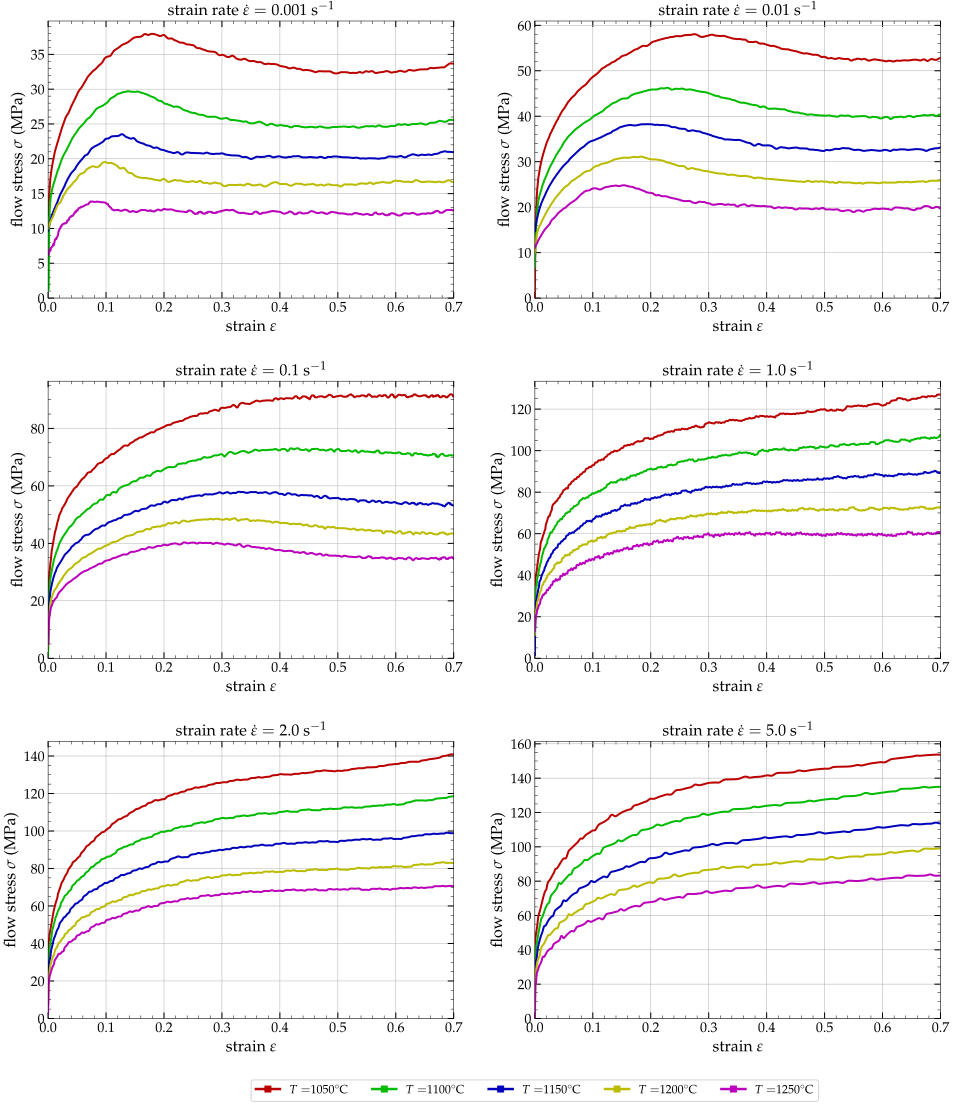
\includegraphics[width=0.9\columnwidth]{Figures/rawData}
\caption{Stress--strain curves of medium carbon alloy extracted from the Gleeble device for 5 temperatures ($T$) and 6 strain rates ($\mdot\varepsilon$).}
\label{fig:RawData}
\end{figure}

The flow stress ($\sigma$) increases with increasing strain rate ($\mdot\varepsilon$) but decreases with increasing temperature ($T$).
It is noteworthy that the flow stress is also influenced by the strain.
For the lowest strain rates, the flow stress increases up-to $\sigma_p$ with the strain until reaching a value of approximately $\varepsilon_p=0.2$ to $0.3$.
Subsequently, it decreases to maintain a relatively constant value throughout the test.
Conversely, for the highest strain rates (above $1~\ps$), the flow stress consistently increases during the entire test duration.
The slight increase in stress at low strain rates with large strain values is due to friction between the sample and the anvil during testing as reported by Galos \eal \cite{Galos-2022}.
This frictional effect becomes more pronounced as lubrication decreases over time.

The initial stress increase observed during deformation up to $\varepsilon=0.1$ is attributed to work hardening (WH).
Subsequently, from $\varepsilon=0.1$ to $0.2$, the flow stress demonstrates a continuous decline as the stress level increases until a peak or inflection point is reached, indicating the dominant influence of thermal softening surpassing work hardening.
At this stage, the stress-strain curve exhibits three different patterns as the strain increases: (i) gradual decrease to a steady state with DRV/DRX softening.
This pattern is observed for all deformation temperatures and strain rates ranging from $\mdot\varepsilon=0.001~\ps$ to $0.1~\ps$, except for those at $1050\celsius$ and $1100\celsius$; (ii) higher stress levels without significant softening and work hardening at $1050\celsius$ and $1100\celsius$ with a strain rate of $0.1~\ps$; (iii) continuous increase with significant work hardening observed for all deformation temperatures and a strain rate of $1~\ps$.
This suggests that softening due to DRX (dynamic recrystallization) occurs at high temperatures and low strain rates.
In contrast, at higher strain rates and lower temperatures, the rate of softening due to DRX is slowed down by higher work hardening rates.
As a result, both the peak stress $\sigma_p$ and the onset of steady-state flow occur at higher strain levels.
The drop in stress observed at all temperatures and strain rates of $\mdot\varepsilon=0.001-5.0~\ps$ is due to the occurrence of DRX.

Dynamic recrystallization is an important phenomenon for controlling the microstructural and mechanical properties of a material during hot working.
In some materials, such as aluminum, dynamic recrystallization can balance work hardening, resulting in the rapid appearance of a plateau.
However, in many austenitic steels, the kinetics of restoration are weak and, as a result, dynamic recrystallization can be triggered at a critical condition of strain accumulation.
Because of the significant influence of dynamic recrystallization on the material's flow stress at high temperature, this inevitably affects the material's microstructure after hot working, and prediction of the critical conditions for the onset of dynamic recrystallization is therefore crucial to good material characterization.
Several factors, such as the chemical composition of the material, the grain size before deformation, the mode of deformation and the deformation parameters (deformation rate, temperature and deformation) condition dynamic recrystallization, which can only be triggered if the critical deformation is reached, and this deformation can be determined using metallography.
However, this technique requires extensive sampling before and after critical deformation.
In addition, phase changes during cooling from the hot working temperature modify the deformed structure, making metallographic analysis difficult.
Hence the need for simpler techniques, such as the development of analytical models.
With this in mind, a number of studies have been carried out to determine analytically the initiation of dynamic recrystallization.

In this paper we will use the Johnson-Mehl-Avrami-Kohnogorov (JMAK) phenomenological model \cite{Avrami-1939} to compute the evolution of DRX of the material during the deformation.
The raw data acquired from the Gleeble thermosimulator will subsequently be used to identify the material flow law and the parameters of the DRX model.

%----------------------------------------------------------------------------------
\subsection{DRX model's parameters identification\label{subsec:DRXParameters}}
%----------------------------------------------------------------------------------

In this Section we will determine the critical deformation required to initiate recrystallization.
Ryan and McQueen \cite{Ryan-1989, Ryan-1990, Ryan-1990-2} were the first to study this phenomenon, observing the appearance of an inflection point on the curve $\theta(\sigma)=\frac{\partial \sigma}{\partial \varepsilon}$ before the peak stress $\sigma_p$ and attributed to this inflection point the start of dynamic recrystallization and therefore the critical values $\varepsilon_c$ and $\sigma_c$ of the strain and the stress respectively.
Later Poliak and Jonas \cite{Poliak-1996, Poliak-2003, Poliak-2003-2, Jonas-2003} further demonstrated that this inflection point is associated with a thermodynamic free energy released during dislocation motion, and consequently endorse the dynamic recrystallization hypothesis describing this inflection point.
Najafizadeh and Jonas \cite{Najafizadeh-2006} simplified the thermodynamic model of Poliak and Jonas by developing an analytical technique, widely used today, to determine the critical conditions for the initiation of dynamic recrystallization.
In their approach, a polynomial of $3^\text{th}$ degree is adopted to describe the shape of the curve $\theta(\sigma)$ and, using the second derivative, they manage to identify the critical stress and strain ($\sigma_c$ and $\varepsilon_c$).

As introduced earlier, the determination of critical values for the initiation of DRX involves determining the inflection point located on the $\theta(\sigma)$ curve between $\varepsilon=0$ and $\varepsilon_c$.
One of the first difficulties is to numerically evaluate the value of the derivative of stress versus strain, since experimental data from compression tests show oscillations, as illustrated in Figure \ref{fig:RawData}.
It is therefore not possible to calculate the derivative $\theta(\sigma)=\frac{\partial \sigma}{\partial \varepsilon}$ directly.

To get around this problem, some authors recommend smoothing the experimental data (using the Excel solver for \cite{Najafizadeh-2006}) or identifying an analytical form (e.g. a polynomial of relatively high order) using a minimization algorithm.
But, depending on the degree of the polynomial and for the same stress/strain curve, several solutions can be obtained, leading to the definition of several possible forms for the $\theta(\sigma)$ function.

%----------------------------------------------------------------------------------
\subsubsection{ANN based filtering method for raw data\label{subsec:ANNbasics}}
%----------------------------------------------------------------------------------
In order to improve the results obtained from the critical value identification procedure, we propose here to use the universal approximator capability of artificial neural networks to replace each strain-hardening curve by its representation in the form of an ANN with 1 input (strain) and 1 output (stress).
In such a network, each layer of neurons is connected to the one before it and the one after it by weighted connections.
Any hidden layer $k$, containing $n$ neurons, takes a weighted sum of the outputs $\overrightarrow{\hat{y}}$ of the immediately preceding layer $(k-1)$, containing $m$ neurons, given by the following~equation:
\begin{equation}
y_i\lay{k} = \sum_{j=1}^m w_{ij}\lay{k} \hat{y}_j^{(k-1)}+ b_i\lay{k},\label{eq:ANN1}
\end{equation}
where $y_i\lay{k}$ is the entry of the  $i$th neuron of layer $k$, $\hat{y}_j\lay{k-1}$ is the output of the $j$th neuron of layer $(k-1)$, $w_{ij}\lay{k}$ is the associated weight parameter between the  $i$th neuron of layer $k$ and the  $j$th neuron of layer $(k-1)$, and $b_i\lay{k}$ is the associated bias of the  $i$th neuron of layer $k$.
Those weights $w_{ij}$ and bias $b_i$, for each layer, are the training parameters of the ANN, which we have to adjust during the training procedure.
For the proposed model, we selected the Sigmoid activation function, so that each neuron in the hidden layer $k$ provides an output value ${\hat{y}}$ from the input value $y$ of the same neuron defined by Equation (\ref{eq:ANN1}) according to the following equation:
\begin{equation}
\hat{y}=\frac{1}{1 + \e{-y}}\label{eq:ANN2}
\end{equation}

No activation function was used for the output neuron of the ANN as usually done in a regression application.
The architecture chosen for our application corresponds to 2 hidden layers of 7 and 5 neurons respectively, as illustrated in Figure \ref{fig:ANN-7-5}.
If $n$ and $m$ are the number of neurons of the first and second hidden layers respectively, the number of internal parameters $N_{int}$ of the model is given by $N_{int}=m(2+n)+2n+1$.
So that for a $7-5$ network, $N_{int}=60$.
\begin{figure}[H]
\centering
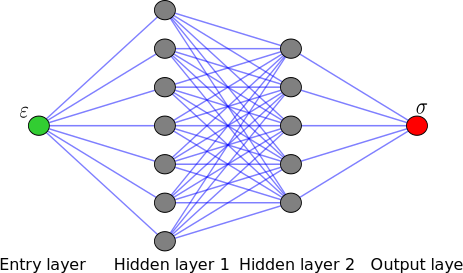
\includegraphics[width=0.7\columnwidth]{Figures/ANN-7-5}
\caption{Two hidden layers artificial neural network architecture with 1 input neuron (green) and 1 output neuron (red).}
\label{fig:ANN-7-5}
\end{figure}
The Python program used for training the neural network was developed using the specialized Python library, Tensorflow \cite{Abadi-2016}.
The Adaptive Moment Estimation (ADAM) optimizer \cite{Kingma-2015} was used for the training phase.

%----------------------------------------------------------------------------------
\subsubsection{ANN filtering results and DRX model parameters evaluation\label{subsec:ANNapplication}}
%----------------------------------------------------------------------------------
Since the DRX occurs only for the 4 strain rates within the range $[0.001~\ps-1.0~\ps]$, we will only use the first 20 stress/strain curves for the DRX critical parameters' identification.
Each of the 20 curves, made up of 701 couples of strain-stress values, was processed independently by a neural network, leading to 20 identified architectures.
As an example, Figure \ref{fig:AnnFit} shows the experimental values of the stress/strain curve for $\mdot\varepsilon=0.001~\ps$ and $T=1050\celsius$ (blue line) and the results from the neural network identified from these data (red line).
\begin{figure}[H]
\centering
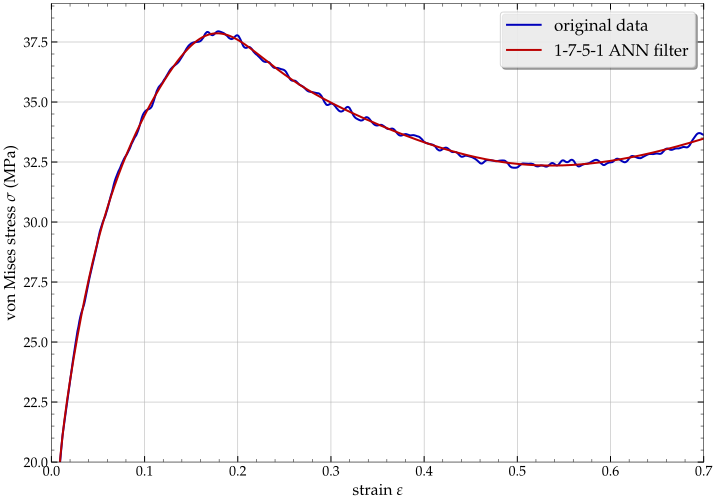
\includegraphics[width=0.7\columnwidth]{Figures/AnnFit}
\caption{Two hidden layers artificial neural network architecture with 1 input neuron (green) and 1 output neuron (red).}
\label{fig:AnnFit}
\end{figure}
The accuracy and predictive ability of the models are usually assessed through certain coefficients such as the mean absolute relative error ($\MARE$) defined by Equation (\ref{eq:AARE}):
\begin{equation}
\MARE(\%) = \frac{1}{N} \sum_{i=1}^{N}{\left|\frac{\sigma_i^p -\sigma_i^e}{\sigma_i^e}\right|} \times 100, \label{eq:AARE}
\end{equation}
and the root-mean-squared error ($\RMSE$) defined by Equation (\ref{eq:RMSE}):
\begin{equation}
\RMSE (\MPa) = \sqrt{\frac{1}{N} \sum_{i=1}^{N} \left(\sigma_i^p - \sigma_i^e\right)^2}, \label{eq:RMSE}
\end{equation}
where $\sigma_i^e$ is the experimental value, $\sigma_i^p$ is the value of the stress $\sigma$ predicted using the given model, and $N$ is the total number of data points used to compute those coefficients.
For the proposed ANN filter $\RMSE=0.093~\MPa$ and $\MARE=0.231~\%$, while using a $11^{th}$ order polynomial fit of the experimental data leads to $\RMSE=0.120~\MPa$ and $\MARE=0.275~\%$.

\begin{figure}[H]
\centering
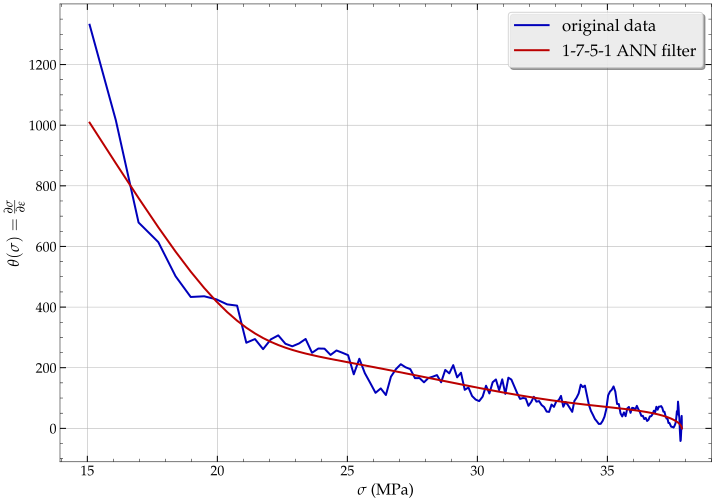
\includegraphics[width=0.7\columnwidth]{Figures/AnnTheta}
\caption{Two hidden layers artificial neural network architecture with 1 input neuron (green) and 1 output neuron (red).}
\label{fig:AnnTheta}
\end{figure}

%\begin{table}[H]
%\caption{Architecture and accuracy coefficients for all the proposed networks.}
%\newcolumntype{C}{>{\centering\arraybackslash}X}
%\newcolumntype{L}{>{\raggedright\arraybackslash}X}
%\begin{tabularx}{\textwidth}{LCCCCCC}
%\hline
%Coefficient & $\mdot\varepsilon$ & $1050\celsius$ & $1100\celsius$ & $1150\celsius$ & $1200\celsius$ & $1250\celsius$  \\
%\hline
%$\MARE(\%)$ & $0.001$ & $0.231$ & $1.13$ & $1.05$ & $1.08$ & $0.75$ \\
%$\RMSE(\MPa)$ & $0.001$ & $0.093$ & $0.59$ & $0.57$ & $0.65$ & $0.46$ \\
%\hline
%\end{tabularx}
%\label{tab:Errors}
%\end{table}

%----------------------------------------------------------------------------------
\section{Numerical simulation of the compression\label{sec:NumSim}}
%----------------------------------------------------------------------------------

%----------------------------------------------------------------------------------
\subsection{Identification of the ANN constitutive law\label{subsec:ANNConstitutiveLaw}}
%----------------------------------------------------------------------------------
In general terms, flow stress $\sigma$ is a non-linear function of the strain $\varepsilon$, increasing with the strain rate $\mdot\varepsilon$, but decreasing with increasing temperature $T$.
The model can therefore be described as an elastoplastic model with the influence of strain rate and temperature.
This type of behavior generally leads to Johnson-Cook \cite{Johnson-1983}, Zerilli Armstrong \cite{Zerilli-1987}, Hansel Spittle \cite{Hensel-1978} or Arrhenius \cite{Sellars-1966} flow law type.
Depending on the nature of the stress-strain relationship, modeling with one or other of these models can take into account the actual behavior of the material at certain strain rates.
As reported by Tize Mha \eal \cite{TizeMha-2023}, Johnson-Cook, Zerilli Armstrong or Hansel Spittle type models, while providing a more or less faithful reproduction of material behavior at strain rates above $1~\ps$, do not take into account the softening due to dynamic recrystallization visible on experimental curves for strain rates below $1~\ps$ as reported in Figure  \ref{fig:RawData}.
Indeed, for the lowest strain rates, the flow stress $\sigma$ increases with strain $\varepsilon$ up to a value of around $\varepsilon=0.2$ to $0.3$ and then decreases to maintain a more or less constant value until the end of the test.
Only the Arrhenius model can more or less account for this softening at low strain rates.
As proposed by Pantalé \eal \cite{Pantale-2021, Pantale-2023} and Tize Mha \eal \cite{TizeMha-2023}, an effective alternative is to use a flow law defined by an artificial neural network trained directly on experimental data from compression tests.
Correctly defining the hyperparameters of this neural network (number of hidden layers, number of neurons, activation functions, etc.) allows us to obtain a flow law that faithfully reproduces the data obtained from compression tests.

According to the method proposed by Pantalé \eal \cite{Pantale-2021, Pantale-2023}, we developed in Tize Mha \eal \cite{TizeMha-2023} a two hidden layers ANN based flow law whose general structure is reported in Figure \ref{fig:ANN-2HL}.
This ANN contains an input layer of three neurons corresponding to the entries of the model ($\varepsilon$, $\mdot\varepsilon$ and $T$), an output layer with one neuron ($\sigma$), and $2$ hidden layers.


All details about the artificial neural network, setup of the experimental data and the training method is reported the paper proposed by Pantalé \cite{Pantale-2023}.
%Thus, all the neurons of the $k^{th}$ layer are connected to all the neurons of the ($k-1^{th}$) layer, as shown in~Figure~\ref{fig:ANN-2HL}.

\begin{figure}[H]
\centering
\includegraphics[width=0.7\columnwidth]{Figures/ANN-scheme-2HL}
\caption{Two hidden layers artificial neural network architecture with 3 inputs neurons (green) and 1 output neuron (red).}
\label{fig:ANN-2HL}
\end{figure}

We again used the Tensorflow library for the development of the training program, and the ADAM optimizer was used for the training phase.
The provided database presented in Section \ref{subsec:ExperimentalProcedure} consists of $21,030$ quadruplets of strain ($\varepsilon$), strain rate ($\mdot\varepsilon$), temperature ($T$) and stress ($\sigma$) values.
%The training data were those from the tests presented in Section \ref{sec:ComTestResults} and were composed of $21,030$ quadruplets of ($\varepsilon$, $\mdot\varepsilon$, $T$, $\sigma$) values.

We selected 6 different networks, named 3-$n$-$m$-1, where $n$ is the number of neurons in the first hidden layer and $m$ is the number of neurons in the second hidden layer, to show the importance of selecting the adequate number of neurons in the two layers.

The training was performed on the basis of $5000$ epochs of the experimental dataset.
It took $40$~min of training on a Dell XPS-13 7390 laptop running Ubuntu 22.04 LTS 64 bits with 16 GB of RAM and an Intel 4-core i7-10510U processor to obtain the converged parameters of the ANN model.

Figure \ref{fig:ANN-conv} shows the evolution of the training error defined by the $\log_{10}$ of the internal $\RMSE$ during the training phase and Table \ref{tab:Errors} summarizes the final values of this criterion, along with the final values of the $\MARE$ and the $\RMSE$ for the 6 configurations of the neural network.
On the basis of those results, we have selected the 3-15-7-1 network for further study, as it has the best convergence evolution and the lowest final error values ($\MARE=0.62\%$ and $\RMSE=0.38~\MPa$), while keeping a reasonable number of internal parameters ($N_{int}=180$).

\begin{figure}[H]
\centering
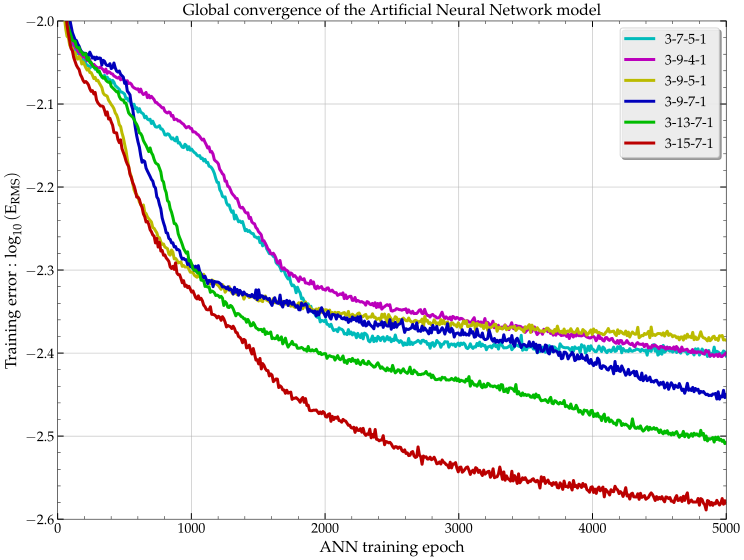
\includegraphics[width=0.7\columnwidth]{Figures/Conv-ANN-6}
\caption{Evolution of the convergence of the models during the training procedure for the 6 proposed network architectures.}
\label{fig:ANN-conv}
\end{figure}

\begin{table}[H]
\caption{Architecture and accuracy coefficients for all the proposed networks.}
\newcolumntype{C}{>{\centering\arraybackslash}X}
\newcolumntype{L}{>{\raggedright\arraybackslash}X}
\begin{tabularx}{\textwidth}{LCCCCCC}
\hline
\textbf{Coefficients} & \textbf{3-7-5-1} & \textbf{3-9-4-1} & \textbf{3-9-5-1} & \textbf{3-9-7-1} & \textbf{3-13-7-1} & \textbf{3-15-7-1} \\
\hline
$N_{int}$ & $74$ & $81$ & $92$ & $114$ & $158$ &$180$\\
\hline
$\log_{10}(\RMSE)$ & $-2.40$ & $-2.42$ & $-2.38$ & $-2.45$ & $-2.50$ & $-2.58$ \\
$\MARE(\%)$ & $1.13$ & $1.05$ & $1.08$ & $0.91$ & $0.75$ & $0.62$ \\
$\RMSE(\MPa)$ & $0.59$ & $0.57$ & $0.65$ & $0.55$ & $0.46$ & $0.38$ \\
\hline
\end{tabularx}
\label{tab:Errors}
\end{table}

\begin{figure}[H]
\centering
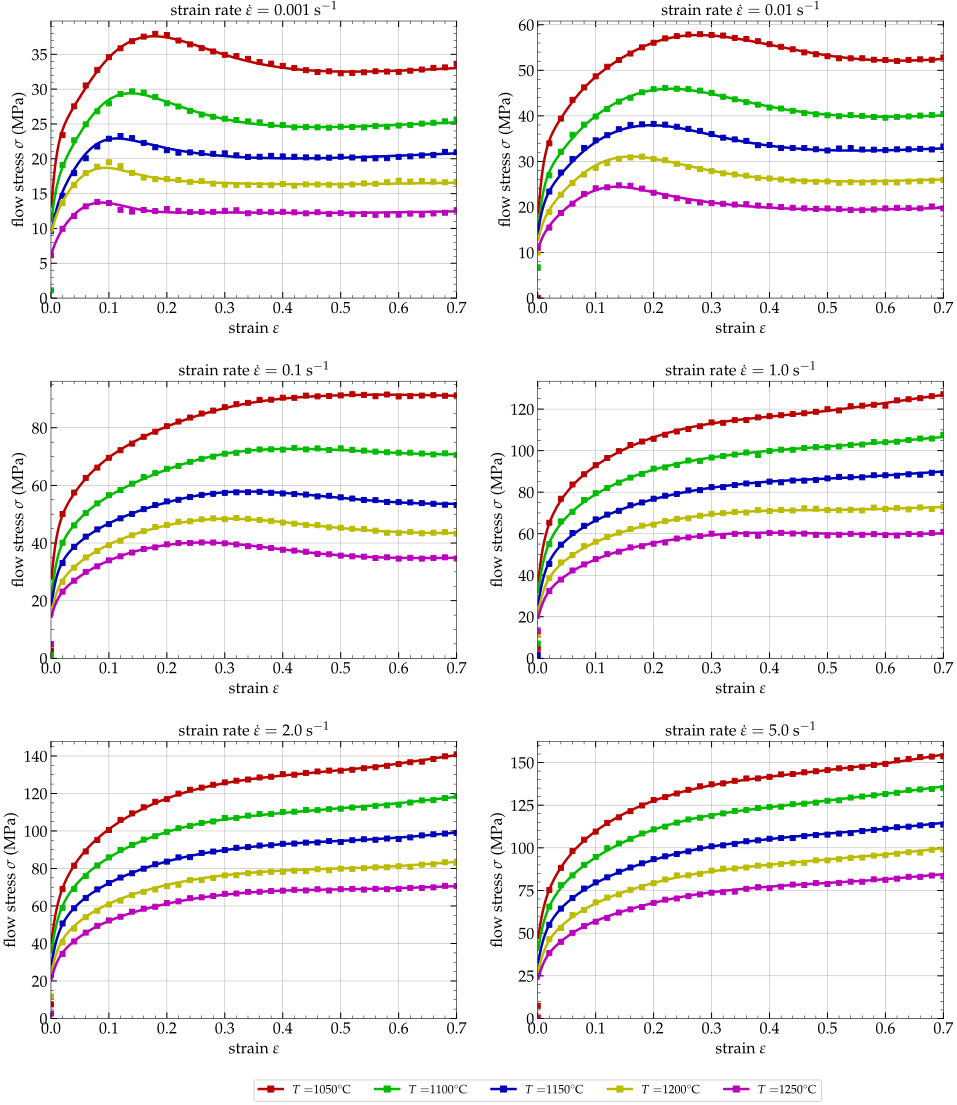
\includegraphics[width=0.9\columnwidth]{Figures/CompExpANN-3-15-7-1}
\caption{Comparison between the experimental (dots) and predicted (lines) flow stresses $\sigma$ by the 3-15-7-1 ANN model.}
\label{fig:ANN-3-15-7-1}
\end{figure}
This model will be used as the material flow law for the numerical simulations presented in Section \ref{subsec:DRXSimulation}.

%----------------------------------------------------------------------------------
\subsection{DRX simulation\label{subsec:DRXSimulation}}
%----------------------------------------------------------------------------------

%----------------------------------------------------------------------------------
\section{Conclusions\label{sec:Conclusions}}
%----------------------------------------------------------------------------------

%%%%%%%%%%%%%%%%%%%%%%%%%%%%%%%%%%%%%%%%%%
%\section{Patents}

%%%%%%%%%%%%%%%%%%%%%%%%%%%%%%%%%%%%%%%%%%
\vspace{6pt}

%%%%%%%%%%%%%%%%%%%%%%%%%%%%%%%%%%%%%%%%%%
%% optional
%\supplementary{The following supporting information can be downloaded at:  \linksupplementary{s1}, Figure S1: title; Table S1: title; Video S1: title.}

% Only for the journal Methods and Protocols:
% If you wish to submit a video article, please do so with any other supplementary material.
% \supplementary{The following supporting information can be downloaded at: \linksupplementary{s1}, Figure S1: title; Table S1: title; Video S1: title. A supporting video article is available at doi: link.}

%%%%%%%%%%%%%%%%%%%%%%%%%%%%%%%%%%%%%%%%%%
\authorcontributions{
Conceptualization, P.T.M. and O.P.;
methodology, O.P.;
software, P.T.M. and O.P.;
validation, O.P.;
formal analysis, O.P.;
investigation, P.D.;
resources, P.D. and M.J.;
data curation, P.T.M. and P.D.;
writing---original draft preparation, P.T.M.;
writing---review and editing, O.P.;
visualization, O.P.;
supervision, M.J., A.T. and O.P.;
project administration, M.J.;
funding acquisition, M.J.
All authors have read and agreed to the published version of the manuscript.}

\funding{This work was supported by the Natural Sciences and Engineering Research Council of Canada (NSERC) in the framework of a Collaborative Research and Development project (CRD) (Grant Number 5364418).}

%\institutionalreview{In this section, you should add the Institutional Review Board Statement and approval number, if relevant to your study. You might choose to exclude this statement if the study did not require ethical approval. Please note that the Editorial Office might ask you for further information. Please add “The study was conducted in accordance with the Declaration of Helsinki, and approved by the Institutional Review Board (or Ethics Committee) of NAME OF INSTITUTE (protocol code XXX and date of approval).” for studies involving humans. OR “The animal study protocol was approved by the Institutional Review Board (or Ethics Committee) of NAME OF INSTITUTE (protocol code XXX and date of approval).” for studies involving animals. OR “Ethical review and approval were waived for this study due to REASON (please provide a detailed justification).” OR “Not applicable” for studies not involving humans or animals.}

%\informedconsent{Any research article describing a study involving humans should contain this statement. Please add ``Informed consent was obtained from all subjects involved in the study.'' OR ``Patient consent was waived due to REASON (please provide a detailed justification).'' OR ``Not applicable'' for studies not involving humans. You might also choose to exclude this statement if the study did not involve humans.
%
%Written informed consent for publication must be obtained from participating patients who can be identified (including by the patients themselves). Please state ``Written informed consent has been obtained from the patient(s) to publish this paper'' if applicable.}

\dataavailability{The raw/processed data required to reproduce these findings cannot be shared at this time due to privacy and ethical concerns.}

\acknowledgments{The authors acknowledge Jean-Benoit Morin, Director of Metallurgy and Quality from Finkl Steel-Sorel, Abdelhalim Loucif from the R\&D department of Finkl Steel-Sorel, Ecole de Technologie Superieure, and Ecole Nationale d'Ingenieurs de Tarbes, France, for providing technical data, materials, and testing facilities.}%MDPI: We removed titles here: OK

\conflictsofinterest{The authors declare no conflict of interest.}

%%%%%%%%%%%%%%%%%%%%%%%%%%%%%%%%%%%%%%%%%%
%% Optional
%\sampleavailability{Samples of the compounds ... are available from the authors.}

%% Only for journal Encyclopedia
%\entrylink{The Link to this entry published on the encyclopedia platform.}

\abbreviations{Abbreviations}{
The following abbreviations are used in this manuscript:\\

\noindent
\begin{tabular}{@{}ll}
ANN & Artificial neural network \\
AR & Arrhenius \\
CPU & Central processing unit \\
DRV & Dynamic recovery\\
DRX & Dynamic recrystallization \\
FEA & Finite element analysis \\
HS & Hansel--Spittel \\
JC & Johnson--Cook \\
MZA & Modified-Zerilli--Armstrong \\
WH & Work hardening \\
ZA & Zerilli--Armstrong
\end{tabular}
}

%%%%%%%%%%%%%%%%%%%%%%%%%%%%%%%%%%%%%%%%%%
%% Optional
\appendixtitles{no} % Leave argument "no" if all appendix headings stay EMPTY (then no dot is printed after "Appendix A"). If the appendix sections contain a heading then change the argument to "yes".
\appendixstart
\appendix
\section[\appendixname~\thesection]{}\label{sec:Appendix}

%%%%%%%%%%%%%%%%%%%%%%%%%%%%%%%%%%%%%%%%%%
\begin{adjustwidth}{-\extralength}{0cm}
%\printendnotes[custom] % Un-comment to print a list of endnotes

\reftitle{References}

% Please provide either the correct journal abbreviation (e.g. according to the “List of Title Word Abbreviations” http://www.issn.org/services/online-services/access-to-the-ltwa/) or the full name of the journal.
% Citations and References in Supplementary files are permitted provided that they also appear in the reference list here.

%=====================================
% References, variant A: external bibliography
%=====================================
\bibliography{bibliography}

% If authors have biography, please use the format below
%\section*{Short Biography of Authors}
%\bio
%{\raisebox{-0.35cm}{\includegraphics[width=3.5cm,height=5.3cm,clip,keepaspectratio]{Definitions/author1.pdf}}}
%{\textbf{Firstname Lastname} Biography of first author}
%
%\bio
%{\raisebox{-0.35cm}{\includegraphics[width=3.5cm,height=5.3cm,clip,keepaspectratio]{Definitions/author2.jpg}}}
%{\textbf{Firstname Lastname} Biography of second author}

% For the MDPI journals use author-date citation, please follow the formatting guidelines on http://www.mdpi.com/authors/references
% To cite two works by the same author: \citeauthor{ref-journal-1a} (\citeyear{ref-journal-1a}, \citeyear{ref-journal-1b}). This produces: Whittaker (1967, 1975)
% To cite two works by the same author with specific pages: \citeauthor{ref-journal-3a} (\citeyear{ref-journal-3a}, p. 328; \citeyear{ref-journal-3b}, p.475). This produces: Wong (1999, p. 328; 2000, p. 475)

%%%%%%%%%%%%%%%%%%%%%%%%%%%%%%%%%%%%%%%%%%
%% for journal Sci
%\reviewreports{\\
%Reviewer 1 comments and authors’ response\\
%Reviewer 2 comments and authors’ response\\
%Reviewer 3 comments and authors’ response
%}
%%%%%%%%%%%%%%%%%%%%%%%%%%%%%%%%%%%%%%%%%%
\PublishersNote{}
\end{adjustwidth}
\end{document}

